\documentclass{beamer}
\usepackage{beamerthemesplit}
\usepackage{wrapfig}
\usetheme{SPbGU}
\usepackage{pdfpages}
\usepackage{amsmath}
\usepackage{cmap}
\usepackage[T2A]{fontenc}
\usepackage[utf8]{inputenc}
\usepackage[english,russian]{babel}
\usepackage{indentfirst}
\usepackage{amsmath}
\usepackage{tikz}
\usepackage{multirow}
\usepackage[noend]{algpseudocode}
\usepackage{algorithm}
\usepackage{algorithmicx}
\usetikzlibrary{shapes,arrows}
\usepackage{fancyvrb}
\newtheorem{rutheorem}{Теорема}
\newtheorem{ruproof}{Доказательство}
\newtheorem{rudefinition}{Определение}
\newtheorem{rulemma}{Лемма}
\beamertemplatenavigationsymbolsempty

% объявляем новую команду для переноса строки внутри ячейки таблицы
\newcommand{\specialcell}[2][c]{%
  \begin{tabular}[#1]{@{}c@{}}#2\end{tabular}}

\title[]{Библиотека GLL парсер-комбинаторов для .NET}
%\subtitle[]{Опциональный подзаголовок}
% То, что в квадратных скобках, отображается в левом нижнем углу.
\institute[СПбГУ]{
Санкт-Петербургский государственный университет \\
Кафедра системного программирования }

% То, что в квадратных скобках, отображается в левом нижнем углу.
\author[Кирилл Мелентьев]{Мелентьев Кирилл Игоревич, 3 курс \\
  % У научного руководителя должна быть указана научная степень
  \and
    {\bfseries Научный руководитель:} ст.пр. С.В. Григорьев \\
  % Для курсовой не обязателен. Должна быть указана должность или ученая степень
  % \and
    % {\bfseries Рецензент:} программист ООО ``Рога и копыта'' И.И. Иванов
    }

\date{18 мая 2016г.}

\definecolor{orange}{RGB}{179,36,31}

\begin{document}
{
% Лого университета или организации, отображается в шапке титульного листа
\begin{frame}
  \begin{center}
  {
\includegraphics[width=1.5cm]{pictures/SPbGU_Logo.png}}
  \end{center}
  \titlepage
\end{frame}
}

\begin{frame}[fragile]
  \transwipe[direction=90]
  \frametitle{Введение}
  \begin{itemize}
    \item Синтаксический анализ
    \item Традиционный подход --- генераторы синтаксических анализаторов
    \begin{itemize}
      \item YACC, ANTLR, ...
    \end{itemize}
    \item Парсер комбинаторы
    \begin{itemize}
      \item Parsec --- классическая библиотека для Haskell
      \item FParsec --- для F\#
      \item gll-combinators --- GLL комбинаторы для Scala
    \end{itemize}
    \item Распространенная проблема парсер-комбинаторов --- отсутствие поддержки леворекурсивных правил в грамматике.
  \end{itemize}
\end{frame}

\begin{frame}[fragile]
  \transwipe[direction=90]
  \frametitle{Обзор существующих решений}
  \begin{table}[H]
  \begin{center}
    \begin{tabular}{p{0.28\linewidth}|c|c|c|c}
      Feature\textbackslash Lib  &  \specialcell{FParsec\\(F\#)}   &  \specialcell{XParsec\\(F\#)}
                                 &  \specialcell{Attoparsec\\(Haskell)}  &  \specialcell{gll-combinators\\(Scala)} \\
      \hline
      Левая рекурсия              &        -       &  -  &  -  &  + \\
      \hline
      Вход абстрактного типа      &        -       &  +  &  -  &  - \\
      \hline
      Инкрементальный анализ      &        -       &  -  &  +  &  - \\
    \end{tabular}
  \end{center}
  \end{table}
\end{frame}

% Обязательный слайд: четкая формулировка цели данной работы и постановка задачи
% Описание выносимых на защиту результатов, процесса или особенностей их достижения и т.д.
\begin{frame}[fragile]
  \transwipe[direction=90]
  \frametitle{Постановка задачи}
  \textbf{Целью} работы является разработка библиотеки парсер-комбинаторов, поддерживающих произвольные КС грамматики для платформы .NET

  \textbf{Задачи}:
  \begin{itemize}
    \item Разработать библиотеку парсер-комбинаторов со следующими свойствами и возможностями:
    \begin{itemize}
      \item Платформа реализации .NET
      \item Поддержка произвольных КС грамматик
      \item Поддержка абстрактного входного типа данных
      \item Возможность инкрементального синтаксического анализа
    \end{itemize}
    \item Провести сравнение производительности с существующими решениями
  \end{itemize}
\end{frame}

\begin{frame}[fragile]
  \transwipe[direction=90]
  \frametitle{Реализация}
  \begin{itemize}
    \item Использован алгоритм GLL
    \begin{itemize}
      \item Позволяет использовать произвольные грамматики
    \end{itemize}
    \item Реализация комбинаторов для инкрементального синтаксического анализа:
    \begin{itemize}
      \item На основе изменяемых структур --- расходует дополнительную память
      \item На основе неизменяемых структур --- не копирует лишних данных, но производительность значительно ниже
    \end{itemize}
  \end{itemize}
\end{frame}

\definecolor{colorscala1}{rgb}{1,0.5,0}

\begin{frame}[fragile]
  \transwipe[direction=90]
  \frametitle{Производительность}
    \begin{itemize}
      \item N ::= N N N | N N | '0'
      \begin{itemize}
        \item \color{colorscala1} FsGll
        \item \color{blue} gll-combinators (Scala)
      \end{itemize}
    \end{itemize}
    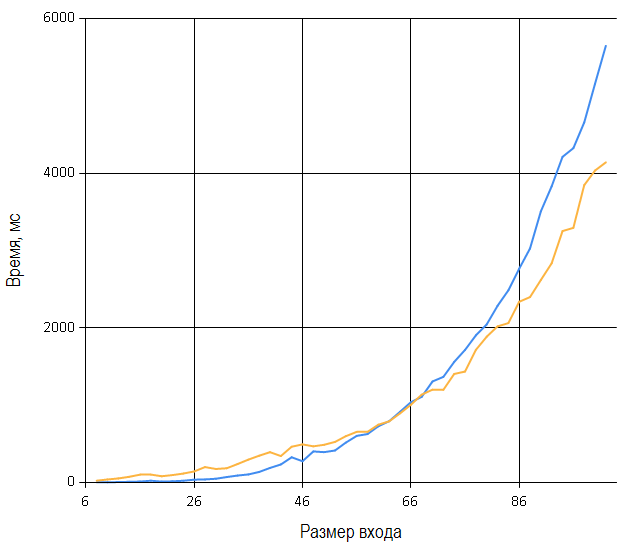
\includegraphics[width=7.6cm]{pictures/graph1.png}
\end{frame}

\begin{frame}[fragile]
  \transwipe[direction=90]
  \frametitle{Производительность}
    \begin{itemize}
      \item ExtCalc %E ::= E ('+'|'-') T | T;  T ::= T ('+'|'-') F | F;  F ::= '-' F | '(' E ')' | num
      \begin{itemize}
        \item \color{blue} FsGll
        \item \color{colorscala1} FParsec
      \end{itemize}
    \end{itemize}
    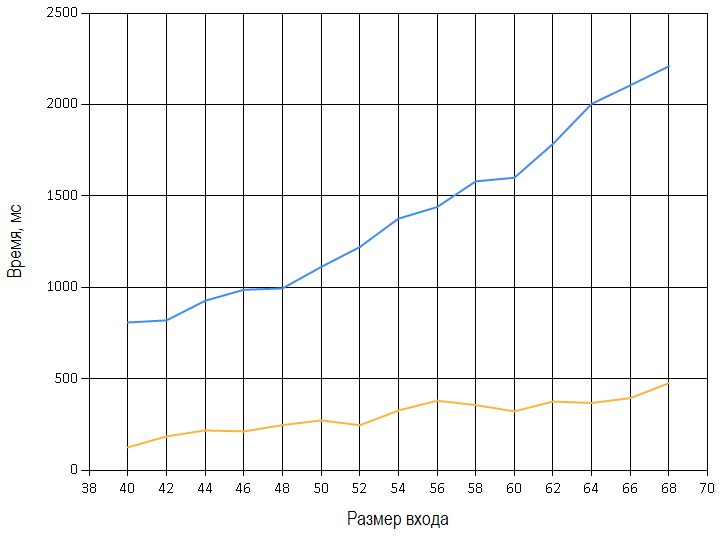
\includegraphics[width=8cm]{pictures/graph2.png}
\end{frame}

\begin{frame}[fragile]
  \transwipe[direction=90]
  \frametitle{Производительность}
    \begin{itemize}
      \item N ::= N N N | N N | '0'
      \begin{itemize}
        \item \color{blue} FsGll, Incremental, Immutable
        \item \color{colorscala1} FsGll, Incremental, Mutable
      \end{itemize}
    \end{itemize}
    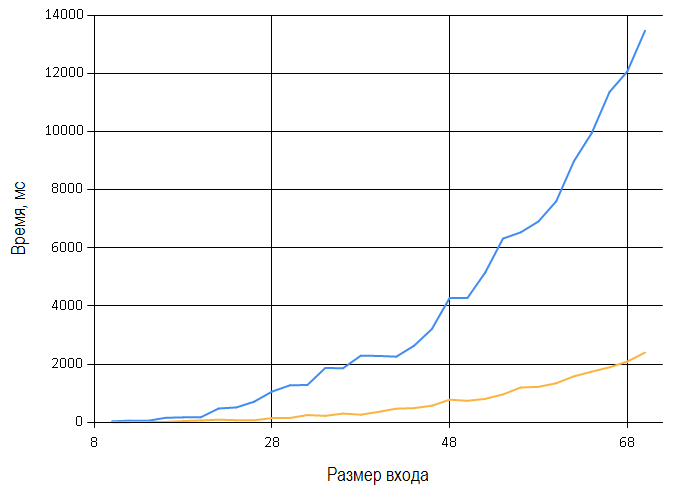
\includegraphics[width=8cm]{pictures/graph3.png}
\end{frame}

\begin{frame}[fragile]
  \transwipe[direction=90]
  \frametitle{Результаты}
  \begin{itemize}
    \item Реализована библиотека парсер-комбинаторов со следующими возможностями и свойствами:
    \begin{itemize}
      \item Платформа реализации .NET
      \item Поддержка произвольных КС грамматик
      \item Поддержка абстрактного входного типа данных
      \item Возможность инкрементального синтаксического анализа
    \end{itemize}
    \item Проведено сравнение производительности с существующими решениями
    \item Выступление с докладом на конференции <<Современные технологии в теории и практике программирования>> в СПбПУ
  \end{itemize}
\end{frame}

\end{document}
